\chapter{Evaluations} 
\label{chap:refs}
\label{chap:ch5_abbr}
\section{Test cases}
We have evaluated this software by testing different functionality as specified in the requirement. This was achieved by creating multiple cases that proves the performance of the software. This evaluation was performed in real time and directly online. We have included images and table showing the test cases and results. 
\section*{Checking Available Machines}
In the software specification section \ref{searchinventory}, it is designed to have search option on the user interface. One of this search requirement is to check for available machines (unreserved machines). In the below table is list of machines reserved for different date. The test is to enter a search query with a specific date interval and ask the software to provide any machine available withing that date.

\begin{table}[h!]
  \centering
  \label{tab:table1}
  \begin{tabular}{l|c||c||c||c||c||c||r}
    No & Machines & Aug & Sep & Oct & Nov & Dec & Jan \\
    \hline
    1 &Machine A & free & free & free & free & free & free\\
    2 &Machine B & free & free & free & 1st to 30th & free & free\\
    3 &Machine C & 17th - & - & - & 24 & free & free\\
    4 &Machine D & 25 & - & 25 & free & free & free\\
    5 &Machine E & free & free & 1st to 31st & free & free & free\\
    6 &Machine F & free & free & free & free & 2nd to 31st & free\\
  \end{tabular}
  \caption{List of Reservations}
\end{table}

\begin{table}[h!]
  \centering
  \label{tab:table1}
  \begin{tabular}{l|c||r}
    No & Date: start --- end & Available machines\\
    \hline
    1 &12-08-2017 to 30-08-2017  & A B E F \\
    2 &17-08-2017 to 24-08-2017  & A B D E F\\
    3 &01-08-2017 to 05-10-2017  & A B F \\
    4 &05-08-2017 to 10-08-2017  & A F \\
    5 &01-08-2017 to 30-08-2017  & A D E  \\
    6 &01-01-2018 to 30-01-2018  & A B C D E F \\
  \end{tabular}
  \caption{test 1}
\end{table}

\begin{table}[h!]
  \centering
  \label{tab:table1}
  \begin{tabular}{l|c||r}
    No & Date: start --- end & Available machines\\
    \hline
    1 &01-08-2017 to 01-01-2018  & A \\
    2 &01-08-2017 to 15-11-2017  & A F\\
    3 &01-12-2017 to 30-01-2018  & B C A D E \\
    4 &30-11-2017 to 30-12-2017  & A  C D E\\
    5 &02-10-2017 to 02-08-2017  & A  D E \\
  \end{tabular}
  \caption{test 2}
\end{table}
\pagebreak
To further explain the reservation process, we have randomly generated different amount of machines and reservation to show a balance evaluation of the reservation process. Figure \autoref{mandr} shows the plot of 10 to 2000 randomly generated reservation on randomly chosen machines.
\begin{figure}
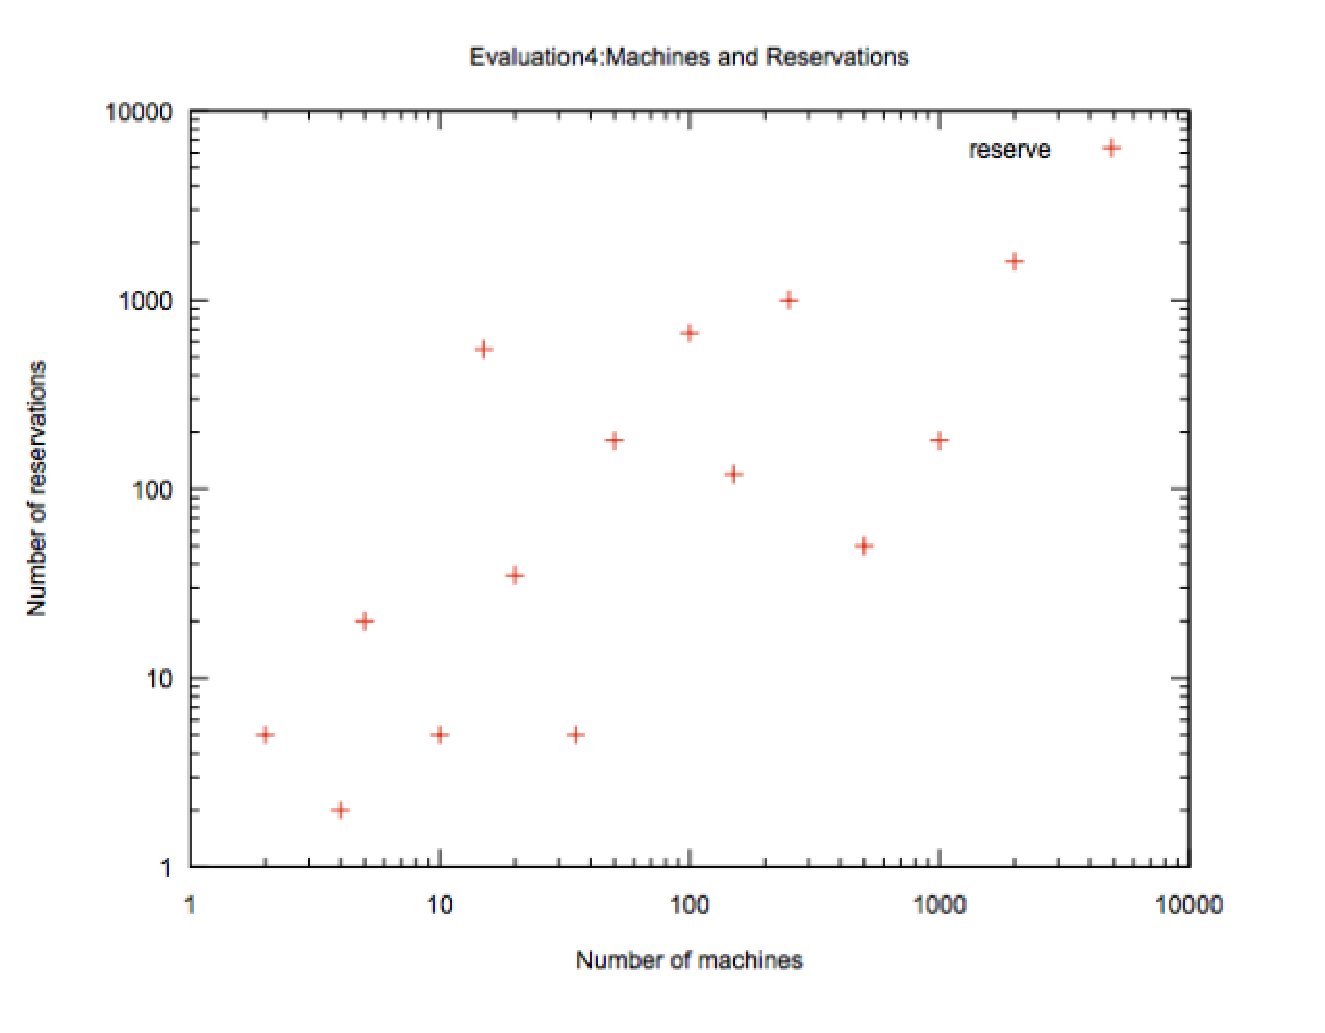
\includegraphics[width=\linewidth]{mandr.eps}
\caption{Scattered plot showing different random generated reservations}
\label{mandr}
\end{figure}

\pagebreak
\section*{Reserving a machine}
Reserving machine is another requirement in section \ref{makereserve} we have implemented in this software. This is the process where users choose and reserve a machine for definite time and date. When a reservation is made, the details of the reservation appears under the machine being reserved. Figure \autoref{reserve} shows the evaluating process of this function, where we put details of reservation, by selecting a user name, machine and inserting start and end time/date. After submitting with the reserve button, the it appears on the inventory with other reservations list. During the testing we tried to input a wrong date and time format and we got an error as shown in figure \autoref{error}. This proved that the software will not take an invalid date format for any reservation process in the system, rather it will issue a warning to the users appropriately.
\begin{figure}[h]
  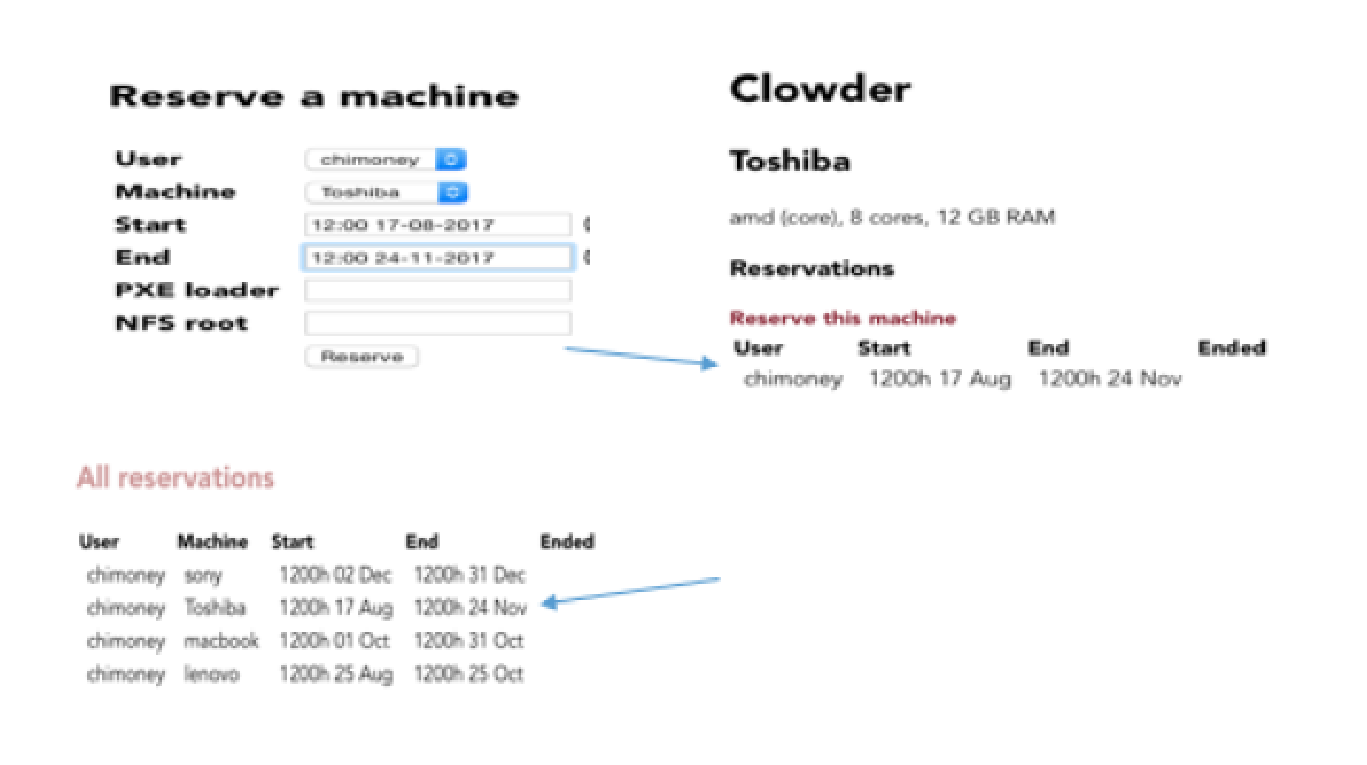
\includegraphics[width=\linewidth]{reserve.eps}
  \caption{Reservation function}
  \label{reserve}
\end{figure}

\begin{figure}
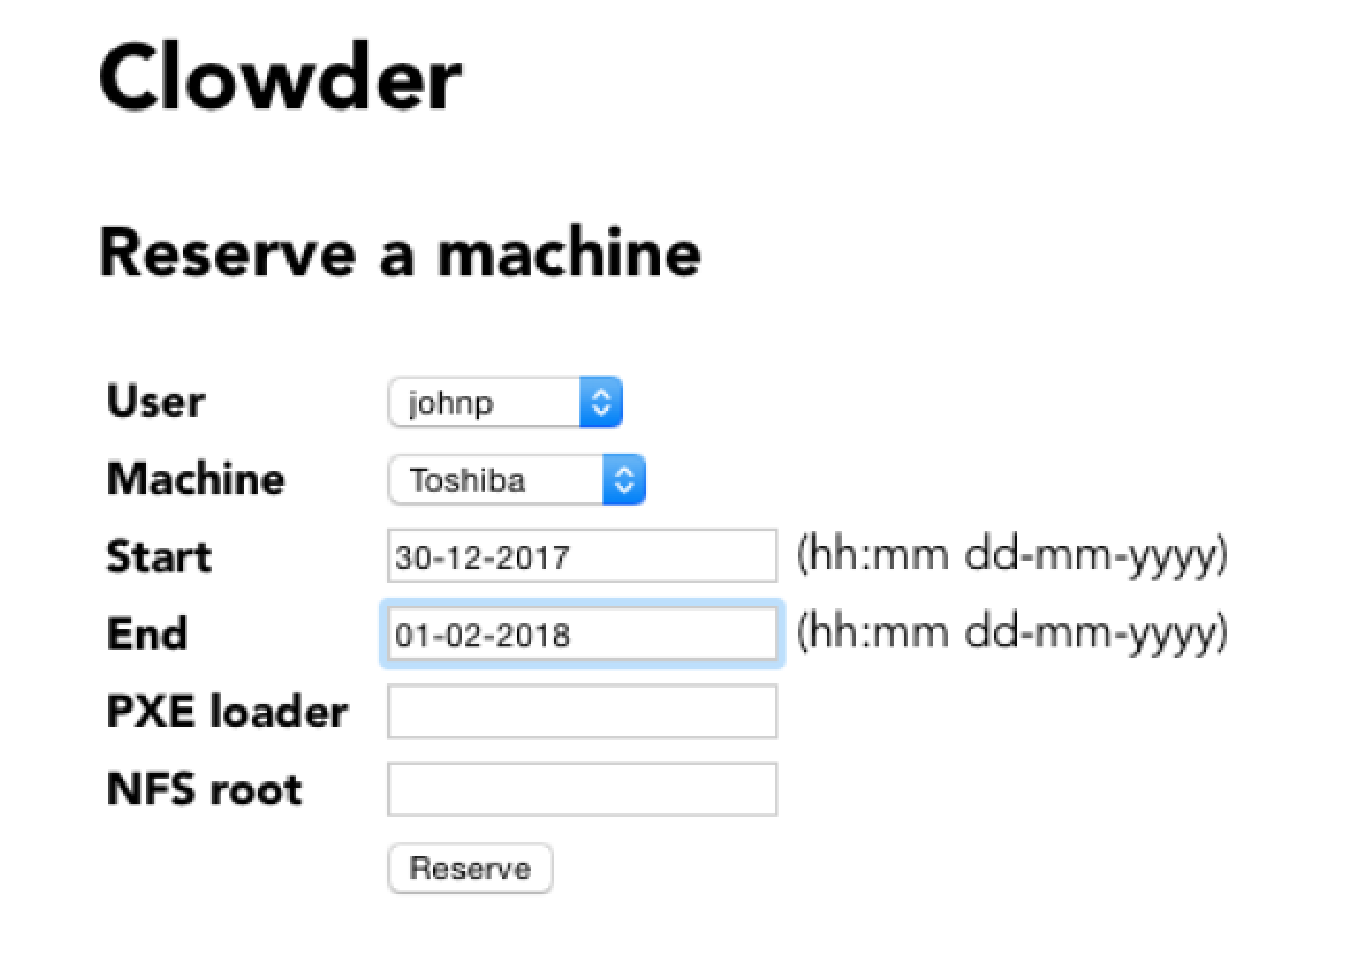
\includegraphics[width=\linewidth]{dateformat1.eps}
\caption{reserving with wrong date}
\end{figure}

\begin{figure}
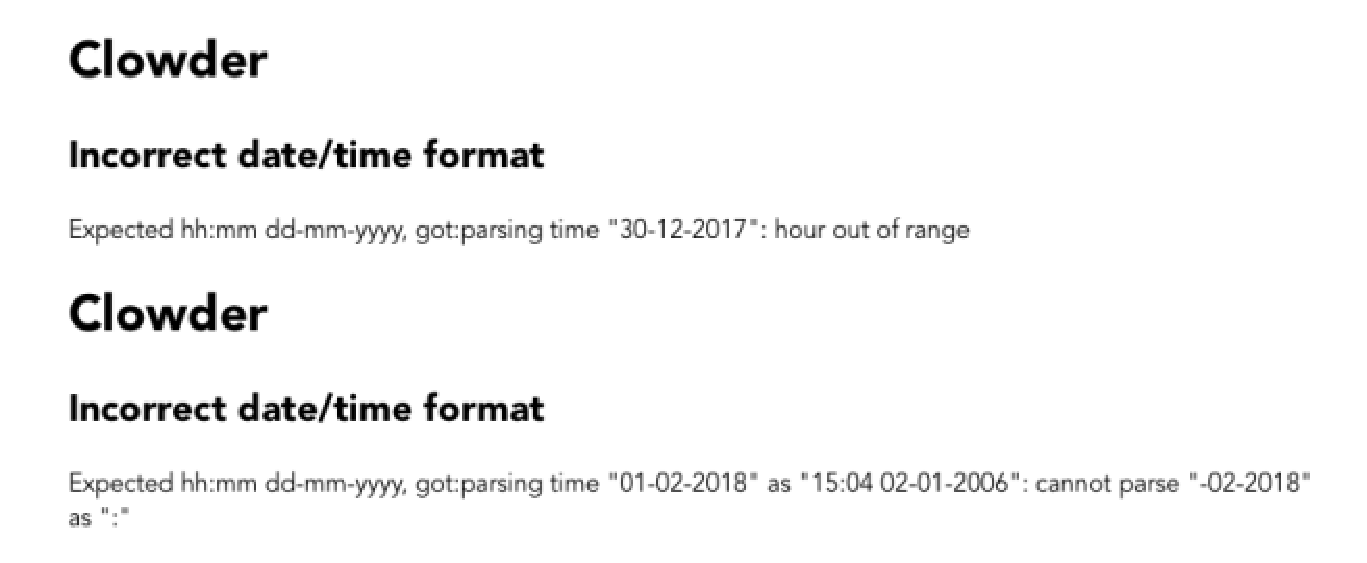
\includegraphics[width=\linewidth]{dateformat2.eps}
\caption{Error message}
\label{error}
\end{figure}

\pagebreak
\section*{Updating a machine}
Update functionality as in section \ref{addmachines} allow users to change the details of a machine already stored in the database. This is to enable them update the information about each machine as needed when ever there is an upgrade in the system. We have tested this functionality by changing the entire information of a machine listed in the inventory. Figure \autoref{update2} shows the process of updating the inventory. This process has proved that this function performed as required because data was collected accordingly and stored with out any error.

\begin{figure}[h]
  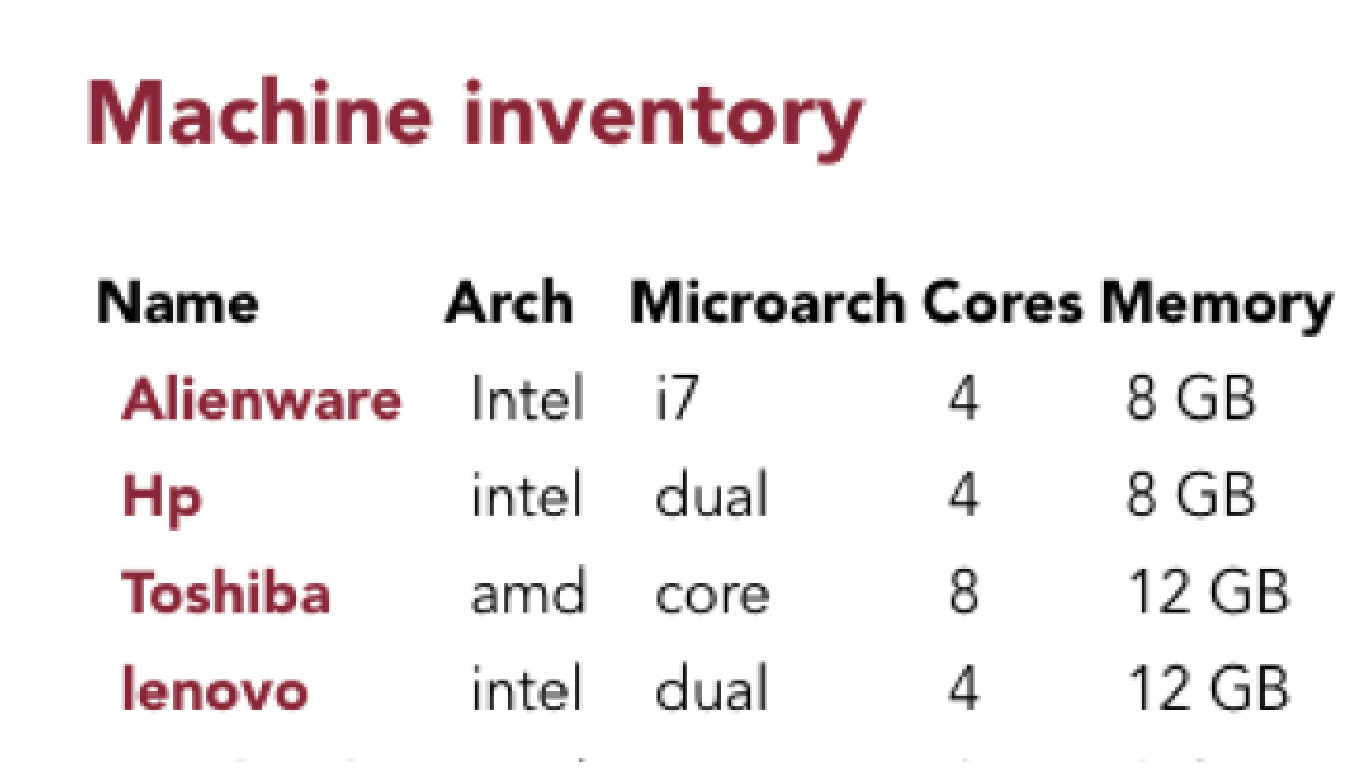
\includegraphics[width=100mm, scale=0.5]{update.eps}
  \caption{Before update}
  \label{update}
\end{figure}
\begin{figure}[h]
  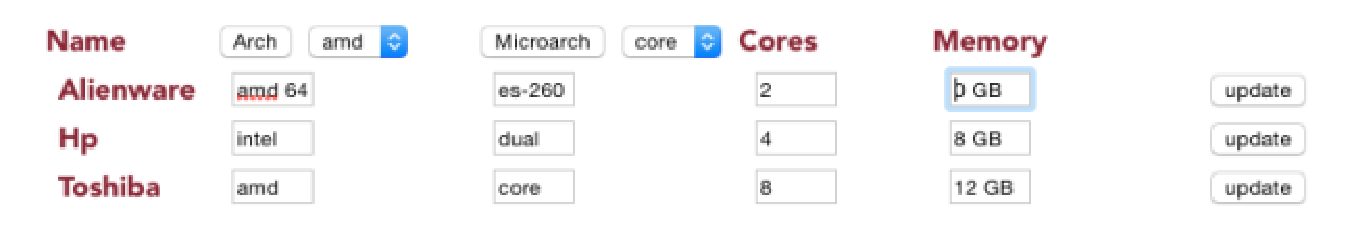
\includegraphics[width=\linewidth]{change.eps}
  \caption{Editing machine details}
   \label{change}
\end{figure}
\begin{figure}[h]
  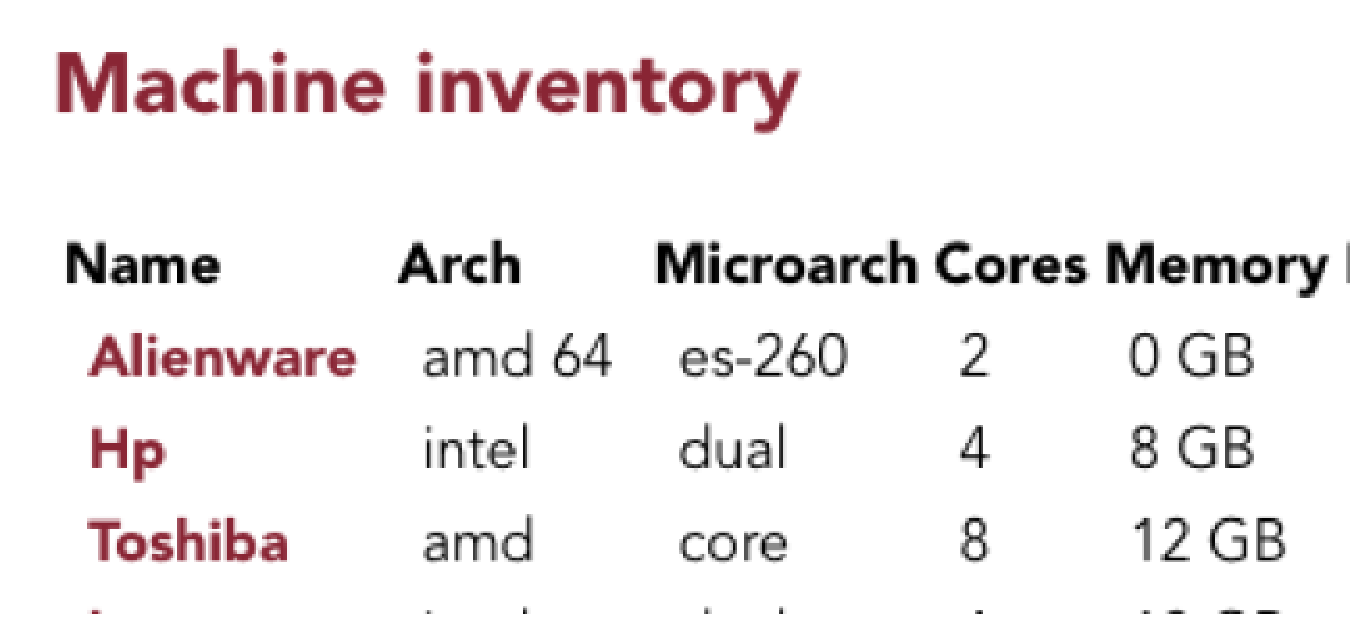
\includegraphics[width=\linewidth]{update2.eps}
  \caption{Updated machine properties}
  \label{update2}
\end{figure}

\pagebreak
\section*{Filtering inventory}
This functionality helps user to filter the inventory using the context of desired information. User is able to filter the machines inventory with memory size. The size range is inserted in the search to get the list of machines that fall within the range. When the button is clicked, the  server returns the list of machine that falls in the range. Another type of filtering is the the drop list filter. This type has a drop down menu user select a context option to search for. For example, user can filter the machine inventory by selecting type OS micro-architecture and architect.
\pagebreak
\pagebreak
\section{Performance Evaluations}
We have evaluated the performance of this software by comparing the performance of the functionality with different sizes of data. The reason for this process is to observe how the software will perform as the system grow in size of machines and other activities. For each requirement tested we recorded their network request speed and the  layout speed. We used random generated data to increase the size of machines from 10 to 1000, and performed this same evaluation accordingly. Figure \autoref{available} shows the performance of the software where we compared the event of searching for a machine in the system. The histogram progress linearly as the data increased. Other figures as well shows same progression, and that means that the performance is steady with a slight change in speed as the system data increases.
\begin{figure}[h]
 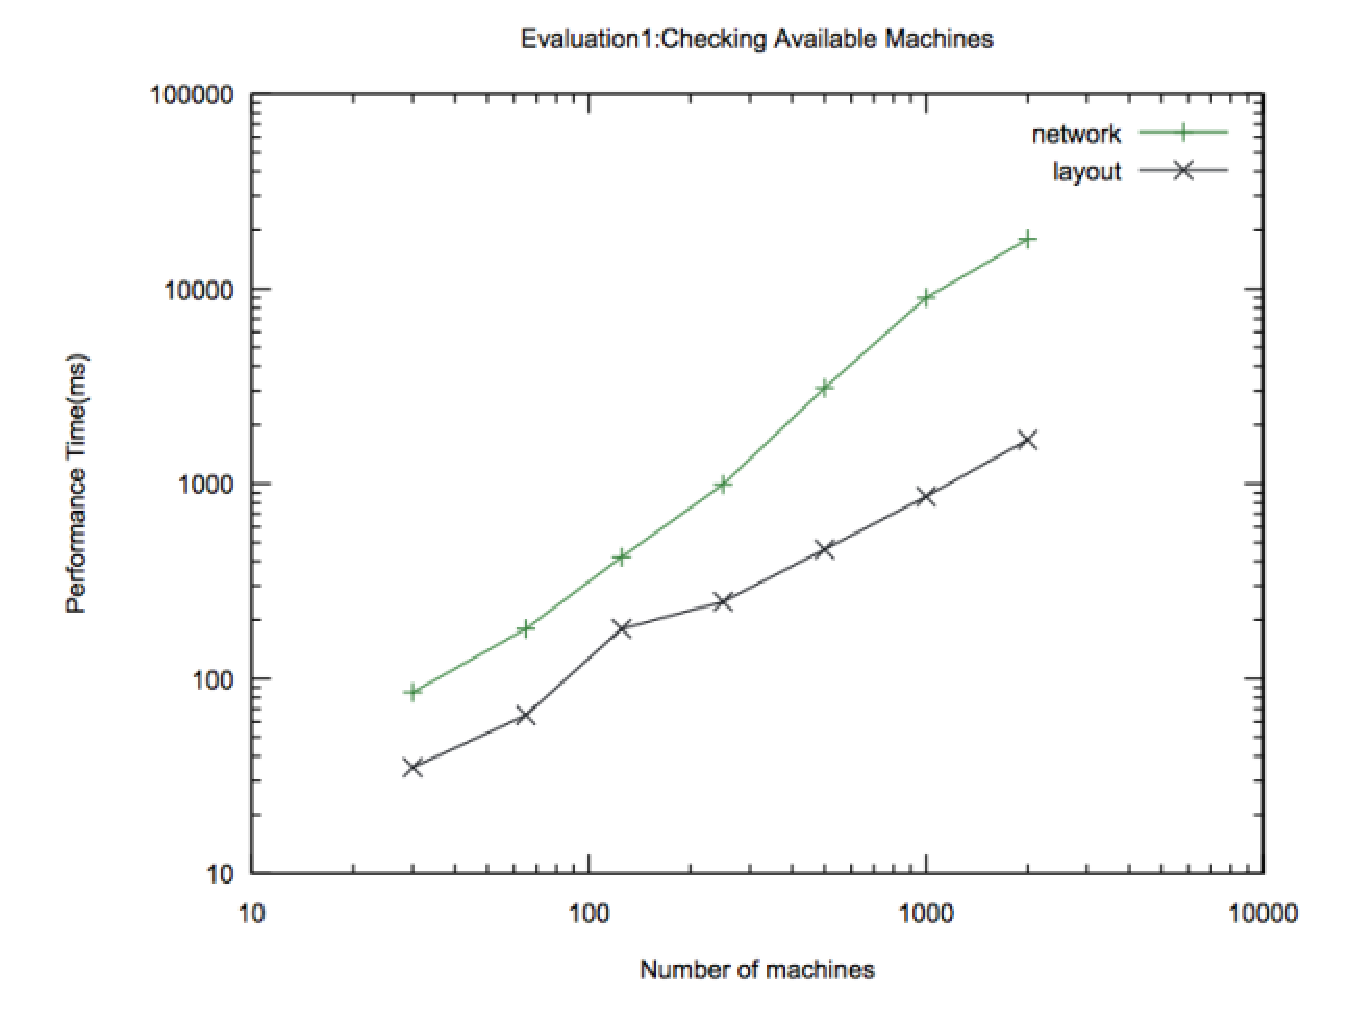
\includegraphics[width=\linewidth]{available.eps}
  \caption{Evaluation of software on searching inventory}
  \label{available}
\end{figure}

\begin{figure}[h]
 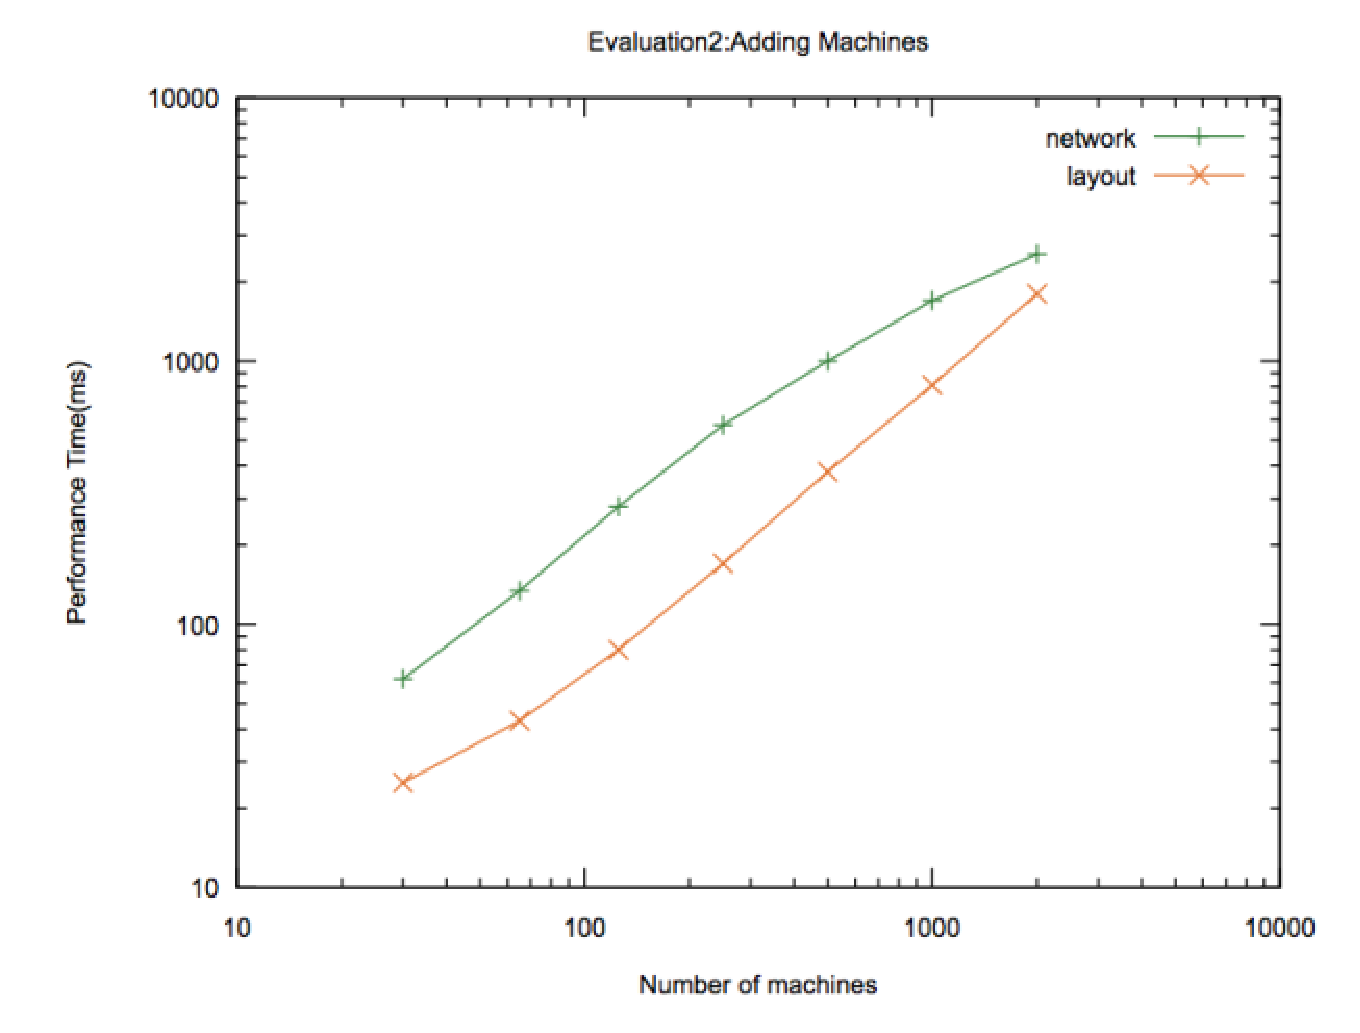
\includegraphics[width=\linewidth]{addmachine.eps}
  \caption{Evaluation of software on adding machines}
  \label{fig:addmachine}
\end{figure}

\begin{figure}[h]
 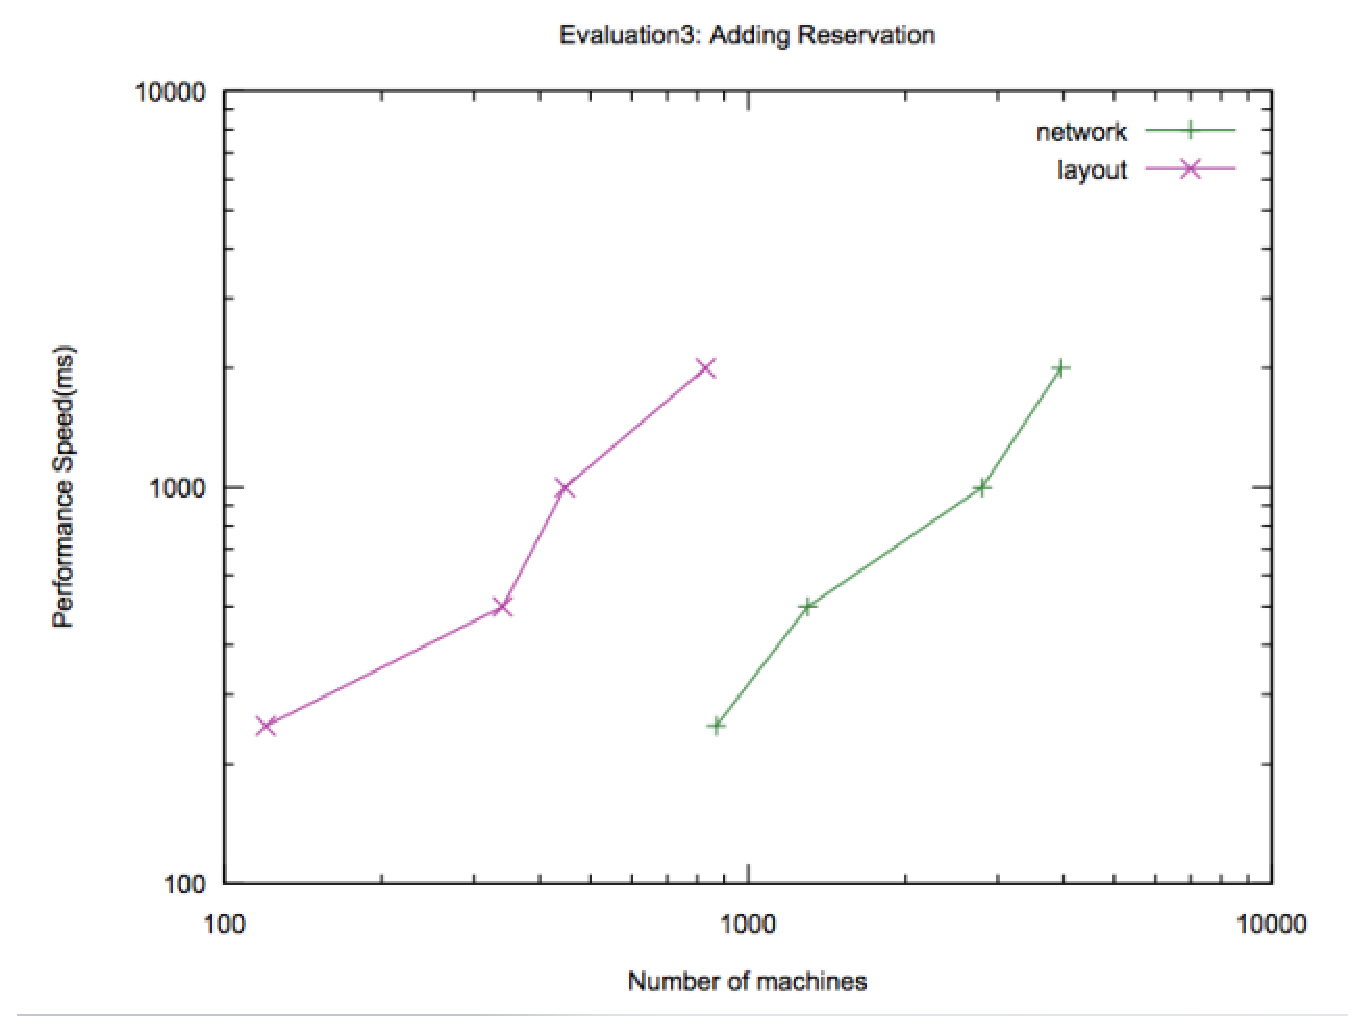
\includegraphics[width=\linewidth]{addreservations.eps}
  \caption{Evaluation of software on making reservation}
\end{figure}